\documentclass{article}
\usepackage{graphicx}
\usepackage{listings}
\usepackage{graphics}
\usepackage[T1]{fontenc}
\usepackage[margin=1.2in]{geometry}
\usepackage{tcolorbox}
\usepackage{hyperref}
\usepackage{dingbat}
\usepackage{float}

\begin{document}

\begin{titlepage}


\title{Multitasking using LPC2148}
\author{e-Yantra Team}
\date{June 2016}
\maketitle
\end{titlepage}




\listoffigures
\tableofcontents
\newpage
\section{Objective}
In this tutorial we will learn how to implement Multitasking using FreeRTOS in Firebird V.
\vspace{3mm}

\section{Prerequisites}
\begin{itemize}
    \item C Programming
    \item Basics of LPC2148
    \item FreeRTOS
\end{itemize}

\section{Hardware Requirements}
\begin{enumerate}
    \item Firebird V (LPC2148)
    \item LCD Interfacing for LPC 2148
    \item Motions control for Firebird V (LPC2148)
    \item Buzzer Operations
\end{enumerate}

\section{Software Requirements}
\begin{itemize}
    \item Keil uvision4
    \item FlashMagic
\end{itemize}

\section{Theory and Description}

\subsection{Motion Control}
\hspace{.5in}
In Firebird V ther are two 75RPM geared motors. The robot can achieve zero turning radius by rotating the two wheels in the opposite direction.
The two motors are driven using the L293D motor driver IC that provides upto 600mA of current.\vspace{.1in}

\hspace{.3in}
Following are the ports that are used to control the motion of the robot and the settings that are required to determine the direction of its motion.

\begin{figure}[h]
\centering
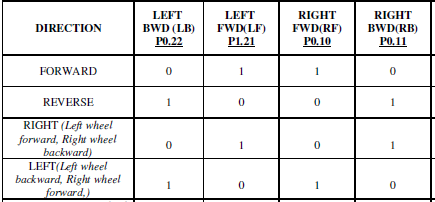
\includegraphics[width=10cm,height=4cm]{motioncontrol.PNG}
\caption{Motion Control Settings}
\end{figure}

\subsection{Buzzer}
In Firebird V 3Khz piezo buzzer is used. It is connected to port P0.25. In order to start and stop the buzzer we can simly use the commands like IO0SET and IO0CLR.  

\begin{figure}[h]
\centering
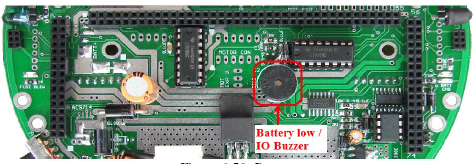
\includegraphics[width=10cm,height=4cm]{buzzer.PNG}
\caption{BUZZER}
\end{figure}

\subsection{LCD Interfacing}
\hspace{.5in}In Firebird V The LCD can be used in 4-bit mode or in 8-bit mode. When used in 8-bit mode it requires 3 control lines and 8 data lines. In order to reduce the number of I/O used we use it 4-bit mode. Here, we only need four data lines.The three control lines used are EN(Enable),RS(Register Select) and R/W(Read/Write)\vspace{.1in}

\hspace{.2in}EN pin : It is used to establish communication between the micro-controller and the LCD. It is connected to port P1.17. In order to transmit data to LCD, we should make sure that firstly it is low and set other control lines as required and then make it high and wait for some time and then make it low again.\vspace{.1in}

\hspace{.2in}RS pin : The RS pin is connected to the port P1.19. When this is set low then the data that is transmitted is treated command that is used for initialisation of LCD and other functions. If it is set high the then the data transmitted is treated as a text data that is to be displayed.\vspace{.1in}
\begin{figure}[h]
\centering
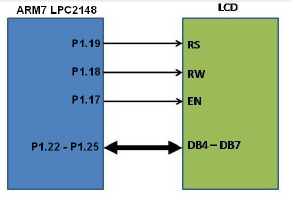
\includegraphics[width=10cm,height=6cm]{LCDconnections.PNG}
\caption{LCD Connections}
\end{figure}


\hspace{.2in}R/W : This pin is connected to port P1.18. If it is set low then it means the data is to be written on LCD. If it is set high then the data is read from LCD.\vspace{.1in}


\hspace{.2in}Ports P1.22-P1.25 are used for data transmission between the LCD and the micro-controller. These line are bi-directional. 

\section{Experiment}

\end{itemize}
\item Use the following code to do Multi-Tasking.\vspace{2mm}
\lstinputlisting[language=C]{rtos_multitasking.c}
\item\textbf{Code Explanation:}
\vspace{2mm}
In the above program, we have created three tasks viz. a buzzer task, a forward motion task and a counter on LCD. These tasks are created using the function "xTaskCreate". Six parameters are defined inside this function.First one is the name of the task that is created as shown in the program. Second is the name of the task in simple terms for the user to understand. Third is the stack size. Fourth parameter is any parameter that we want to pass to that particular task. Fifth is the task priority. We use variable priority in the given example. Last parameter is the name of the taskhandle. Its similar to a pointer. This handle will point to that particular task.\\
The vTaskStartScheduler is the function that schedules the task according to the priority.\\
VTaskDelay is delay generated in terms of ms. It will temporarily suspend that particular task for the defined duration.

\end{enumerate}







\end{document}
